\documentclass[
11pt, % The default document font size, options: 10pt, 11pt, 12pt
codirector, % Uncomment to add a codirector to the title page
]{charter} 


% El títulos de la memoria, se usa en la carátula y se puede usar el cualquier lugar del documento con el comando \ttitle
\titulo{Sistema de monitoreo y gestión remota de sensores Bluetooth para el control del clima en invernaderos} 

% Nombre del posgrado, se usa en la carátula y se puede usar el cualquier lugar del documento con el comando \degreename
%\posgrado{Carrera de Especialización en Sistemas Embebidos} 
\posgrado{Carrera de Especialización en Internet de las Cosas} 
%\posgrado{Carrera de Especialización en Inteligencia Artificial}
%\posgrado{Maestría en Sistemas Embebidos} 
%\posgrado{Maestría en Internet de las cosas}
% IMPORTANTE: no omitir titulaciones ni tildación en los nombres, también se recomienda escribir los nombres completos (tal cual los tienen en su documento)
% Tu nombre, se puede usar el cualquier lugar del documento con el comando \authorname
\autor{Lic. Martín Anibal Lacheski}

% El nombre del director y co-director, se puede usar el cualquier lugar del documento con el comando \supname y \cosupname y \pertesupname y \pertecosupname
\director{Mg. Lic. Leopoldo Alfredo Zimperz}
\pertenenciaDirector{FIUBA} 
\codirector{Dra. Lic. Nancy Beatriz Ganz} % para que aparezca en la portada se debe descomentar la opción codirector en los parámetros de documentclass
\pertenenciaCoDirector{UNaM}

% Nombre del cliente, quien va a aprobar los resultados del proyecto, se puede usar con el comando \clientename y \empclientename
\cliente{Pablo Lodetti}
\empresaCliente{Wentux}
 
\fechaINICIO{20 de agosto de 2024}		%Fecha de inicio de la cursada de GdP \fechaInicioName
\fechaFINALPlan{8 de octubre de 2024} 	%Fecha de final de cursada de GdP
\fechaFINALTrabajo{23 de junio de 2025}	%Fecha de defensa pública del trabajo final


\begin{document}

\maketitle
\thispagestyle{empty}
\pagebreak


\thispagestyle{empty}
{\setlength{\parskip}{0pt}
\tableofcontents{}
}
\pagebreak


\section*{Registros de cambios}
\label{sec:registro}


\begin{table}[ht]
\label{tab:registro}
\centering
\begin{tabularx}{\linewidth}{@{}|c|X|c|@{}}
\hline
\rowcolor[HTML]{C0C0C0} 
Revisión & \multicolumn{1}{c|}{\cellcolor[HTML]{C0C0C0}Detalles de los cambios realizados} & Fecha      \\ \hline
0      & Creación del documento                                 &\fechaInicioName \\ \hline
1      & Se completa hasta el punto 5 inclusive                & {2} de {septiembre} de 2024 \\ \hline
%2      & Se completa hasta el punto 9 inclusive
%		  Se puede agregar algo más \newline
%		  En distintas líneas \newline
%		  Así                                                    & {día} de {mes} de 202X \\ \hline
%3      & Se completa hasta el punto 12 inclusive                & {día} de {mes} de 202X \\ \hline
%4      & Se completa el plan	                                 & {día} de {mes} de 202X \\ \hline

% Si hay más correcciones pasada la versión 4 también se deben especificar acá

\end{tabularx}
\end{table}

\pagebreak



\section*{Acta de constitución del proyecto}
\label{sec:acta}

\begin{flushright}
Buenos Aires, \fechaInicioName
\end{flushright}

\vspace{2cm}

Por medio de la presente se acuerda con el \authorname\hspace{1px} que su Trabajo Final de la \degreename\hspace{1px} se titulará ``\ttitle'' y 
consistirá en {el desarrollo de un sistema de control remoto de clima en invernaderos mediante sensores inalámbricos Bluetooth}. 
El trabajo tendrá un presupuesto preliminar estimado de \textcolor{red}{600} horas y un costo estimado de \textcolor{red}{\$ XXX}, 
con fecha de inicio el \fechaInicioName\hspace{1px} y fecha de presentación pública el \fechaFinalName.

Se adjunta a esta acta la planificación inicial.

\vfill

% Esta parte se construye sola con la información que hayan cargado en el preámbulo del documento y no debe modificarla
\begin{table}[ht]
\centering
\begin{tabular}{ccc}
\begin{tabular}[c]{@{}c@{}}Dr. Ing. Ariel Lutenberg \\ Director posgrado FIUBA\end{tabular} & \hspace{2cm} & \begin{tabular}[c]{@{}c@{}}\clientename \\ \empclientename \end{tabular} \vspace{2.5cm} \\ 
\multicolumn{3}{c}{\begin{tabular}[c]{@{}c@{}} \supname \\ Director del Trabajo Final\end{tabular}} \vspace{2.5cm} \\
\end{tabular}
\end{table}




\section{1. Descripción técnica-conceptual del proyecto a realizar}
\label{sec:descripcion}

\begin{consigna}{red} % El bloque "consigna" se usa para poner texto en rojo y dar una pequeña ayuda sobre cómo completar la sección. 
	%En cada entrega parcial deben eliminar los comandos begin y end del bloque consigna de las secciones que hayan completado.
El objetivo es que el lector, en una o dos páginas, exponga de qué se trata el proyecto y cuáles son sus desafíos, cuál es la motivación para realizarlo y su importancia.

Se debe introducir el contexto del proyecto, el estado del arte en la temática, describir la propuesta de valor, cuál es el problema que atiende y cuál es la solución que se propone. Se debe dar una descripción funcional de la solución que incluya un diagrama en bloques.

Puede ser útil incluir en esta sección la respuesta a alguna de estas preguntas:

\begin{itemize}
	\item ¿Cuál es el contexto del proyecto, es un emprendimiento personal, un proyecto para una empresa, es parte del programa de vinculación con empresas del posgrado?
	\item ¿Existen o aplican condiciones especiales al proyecto, financiamiento de algún programa público o privado, acuerdos de confidencialidad, acuerdos sobre la propiedad intelectual de los entregables u otros?
	\item ¿Cómo se compara la solución propuesta con el estado del arte en el campo de aplicación? ¿En qué aspectos destaca?
	\item ¿Ayuda a la explicación si se incluye un lienzo Canvas del Modelo de Negocio?
	\item ¿En qué estado del ciclo de vida está la solución que se propone?
	\item ¿Cuáles son las características del cliente (el adoptante de los entregables del proyecto) qué valora, qué necesita?
	\item ¿Por dónde pasa la innovación?
\end{itemize}

La descripción técnica-conceptual \textbf{debe incluir al menos un diagrama en bloques del sistema} y descripción funcional de la solución propuesta.

Las figuras se deben mencionar en el texto ANTES de que aparezcan con una frase como la siguiente: ``En la figura \ref{fig:diagBloques} se presenta el diagrama en bloques del sistema. Se observa que...''.  La regla es que las figuras nunca pueden ir antes de ser mencionadas en el texto, porque sino el lector no entiende por qué de pronto aparece una figura.

\begin{figure}[htpb]
\centering 
\includegraphics[width=.65\textwidth]{./Figuras/diagBloques.png}
\caption{Diagrama en bloques del sistema.}
\label{fig:diagBloques}
\end{figure}

\vspace{25px}

El tamaño del texto en TODAS las figuras debe ser adecuado \textbf{para que NO pase lo que ocurre en la figura \ref{fig:diagBloques}}, donde el lector debe esforzarse para poder leer el texto. 

Los colores usados en el diagrama deben ser adecuados, tal que ayuden a comprender mejor el diagrama. Se recomienda evitar colores primarios (como rojo, verde o cyan) y usar la gama de colores pastel.
\end{consigna}

\section{2. Identificación y análisis de los interesados}
\label{sec:interesados}

\begin{consigna}{red} % este comando se debe borrar para la entrega, junto con la contraparte \end{consigna}{red} 
\textbf{Nota importante:} borrar esto y todas las consignas en color rojo antes de entregar este documento). Esto se hace eliminando el par de comandos que forman el bloque consigna, \verb!\begin{consigna}{red}! y \verb!\end{consigna}{red}! del código. 
 
Es inusual que una misma persona esté en más de un rol, incluso en proyectos chicos. Si se considera que una persona cumple dos o más roles, entonces \textbf{solo dejarla en el rol más importante}. 

Por ejemplo, si una persona es Cliente pero también colabora u orienta, dejarla solo como Cliente. Si una persona es el Responsable, \textbf{no debe ser colocado también como miembro del equipo}.


\begin{table}[ht]
%\caption{Identificación de los interesados}
%\label{tab:interesados}
\begin{tabularx}{\linewidth}{@{}|l|X|X|l|@{}}
\hline
\rowcolor[HTML]{C0C0C0} 
Rol           & Nombre y Apellido & Organización 	& Puesto 	\\ \hline
Auspiciante   &                   &              	&        	\\ \hline
Cliente       & \clientename      &\empclientename	&        	\\ \hline
Impulsor      &                   &              	&        	\\ \hline
Responsable   & \authorname       & FIUBA        	& Alumno 	\\ \hline
Colaboradores &                   &              	&        	\\ \hline
Orientador    & \supname	      & \pertesupname 	& Director del Trabajo Final \\ \hline
Equipo        & miembro1 \newline 
				miembro2          &              	&        	\\ \hline
Opositores    &                   &              	&        	\\ \hline
Usuario final &                   &              	&        	\\ \hline
\end{tabularx}
\end{table}

El Director suele ser uno de los orientadores.

No dejar celdas vacías; si no hay nada que poner en una celda colocar un signo ``-''.

No dejar filas vacías; si no hay nada que poner en una fila entonces eliminarla.

Es deseable listar a continuación las principales características de cada interesado.
 
Por ejemplo:
\begin{itemize}
	\item Orientador: la Dra. Ing. María Gómez es experta en la temática y va a ayudar con la definición de los requerimientos y el desarrollo del firmware del embebido.
	\item Auspiciante: es riguroso y exigente con la rendición de gastos. Tener mucho cuidado con esto.
	\item Equipo: Juan Perez, suele pedir licencia porque tiene un familiar con una enfermedad. Planificar considerando esto.
\end{itemize}

\end{consigna} % este comando se debe borrar para la entrega, junto con la contraparte \begin{consigna}{red}


\section{3. Propósito del proyecto}
\label{sec:proposito}

\begin{consigna}{red}
¿Por qué se hace el proyecto? ¿Qué se quiere lograr? 

Se recomienda que sea solo un párrafo que continúe con la idea de la frase ``el propósito de este proyecto es...'' (omitir la frase, ya que está en el título de la sección).
\end{consigna}

\section{4. Alcance del proyecto}
\label{sec:alcance}

\begin{consigna}{red}
¿Qué se incluye y que no se incluye en este proyecto?

Se refiere al trabajo que se va a hacer para entregar el producto o resultado especificado. 

Explicitar todo lo quede comprendido dentro del alcance del proyecto. Por ejemplo:

El proyecto incluye:
\begin{itemize}
	\item Ítem 1.
	\item Ítem 2.
		\begin{itemize}
		\item Subítem 1.
		\item Subítem 2.
		\item ...
		\end{itemize}
	\item ...
	
\end{itemize}

Explicitar además todo lo que no quede incluido (``El presente proyecto no incluye...'')

\end{consigna}


\section{5. Supuestos del proyecto}
\label{sec:supuestos}

\begin{consigna}{red}
``Para el desarrollo del presente proyecto se supone que: ...''

\begin{itemize}
	\item Supuesto 1.
	\item Supuesto 2.
	\item ...
\end{itemize}

Por ejemplo, se podrían incluir supuestos respecto a disponibilidad de tiempo y recursos humanos y materiales, sobre la factibilidad técnica de distintos aspectos del proyecto, sobre otras cuestiones que sean necesarias para el éxito del proyecto como condiciones macroeconómicas o reglamentarias.
\end{consigna}

\section{6. Requerimientos}
\label{sec:requerimientos}

\begin{consigna}{red}
Los requerimientos deben enumerarse y de ser posible estar agrupados por afinidad, por ejemplo:

\begin{enumerate}
	\item Requerimientos funcionales:
		\begin{enumerate}
			\item El sistema debe...
			\item Tal componente debe...
			\item El usuario debe poder...
		\end{enumerate}
	\item Requerimientos de documentación:
		\begin{enumerate}
			\item Requerimiento 1.
			\item Requerimiento 2 (prioridad menor)
		\end{enumerate}
	\item Requerimiento de testing...
	\item Requerimientos de la interfaz...
	\item Requerimientos interoperabilidad...
	\item etc...
\end{enumerate}

Leyendo los requerimientos se debe poder interpretar cómo será el proyecto y su funcionalidad.

Indicar claramente cuál es la prioridad entre los distintos requerimientos y si hay requerimientos opcionales. 

\textbf{¡¡¡No olvidarse de que los requerimientos incluyen a las regulaciones y normas vigentes!!!}

Y al escribirlos seguir las siguientes reglas:
\begin{itemize}
	\item Ser breve y conciso (nadie lee cosas largas). 
	\item Ser específico: no dejar lugar a confusiones.
	\item Expresar los requerimientos en términos que sean cuantificables y medibles.
\end{itemize}

\end{consigna}

\section{7. Historias de usuarios (\textit{Product backlog})}
\label{sec:backlog}

\begin{consigna}{red}
Descripción: en esta sección se deben incluir las historias de usuarios y su ponderación (\textit{history points}). Recordar que las historias de usuarios son descripciones cortas y simples de una característica contada desde la perspectiva de la persona que desea la nueva capacidad, generalmente un usuario o cliente del sistema. La ponderación es un número entero que representa el tamaño de la historia comparada con otras historias de similar tipo.

Se debe indicar explícitamente el criterio para calcular los \textit{story points} de cada historia.

El formato propuesto es: 
\begin{enumerate}
\item ``Como [rol] quiero [tal cosa] para [tal otra cosa]."

\textit{Story points}: 8 (complejidad: 3, dificultad: 2, incertidumbre: 3)
\end{enumerate}
\end{consigna}

\section{8. Entregables principales del proyecto}
\label{sec:entregables}

\begin{consigna}{red}
Los entregables del proyecto son (ejemplo):

\begin{itemize}
	\item Manual de usuario.
	\item Diagrama de circuitos esquemáticos.
	\item Código fuente del firmware.
	\item Diagrama de instalación.
	\item Memoria del trabajo final.
	\item etc...
\end{itemize}
\end{consigna}

\section{9. Desglose del trabajo en tareas}
\label{sec:wbs}

\begin{consigna}{red}
El WBS debe tener relación directa o indirecta con los requerimientos.  Son todas las actividades que se harán en el proyecto para dar cumplimiento a los requerimientos. Se recomienda mostrar el WBS mediante una lista indexada:

\begin{enumerate}
\item Grupo de tareas 1 (suma h)
	\begin{enumerate}
	\item Tarea 1 (tantas h)
	\item Tarea 2 (tantas h)
	\item Tarea 3 (tantas h)
	\end{enumerate}
\item Grupo de tareas 2 (suma h)
	\begin{enumerate}
	\item Tarea 1 (tantas h)
	\item Tarea 2 (tantas h)
	\item Tarea 3 (tantas h)
	\end{enumerate}
\item Grupo de tareas 3 (suma h)
	\begin{enumerate}
	\item Tarea 1 (tantas h)
	\item Tarea 2 (tantas h)
	\item Tarea 3 (tantas h)
	\item Tarea 4 (tantas h)
	\item Tarea 5 (tantas h)
	\end{enumerate}
\end{enumerate}

Cantidad total de horas: tantas.

\textbf{¡Importante!:} la unidad de horas es h y va separada por espacio del número. Es incorrecto escribir ``23hs".

\textbf{Se recomienda que no haya ninguna tarea que lleve más de 40 h.} De ser así se recomienda dividirla en tareas de menor duración.

\end{consigna}

\section{10. Diagrama de Activity On Node}
\label{sec:AoN}

\begin{consigna}{red}
Armar el AoN a partir del WBS definido en la etapa anterior.

Una herramienta simple para desarrollar los diagramas es el Draw.io (\url{https://app.diagrams.net/}).
\href{https://app.diagrams.net}{Draw.io}


\begin{figure}[htpb]
\centering 
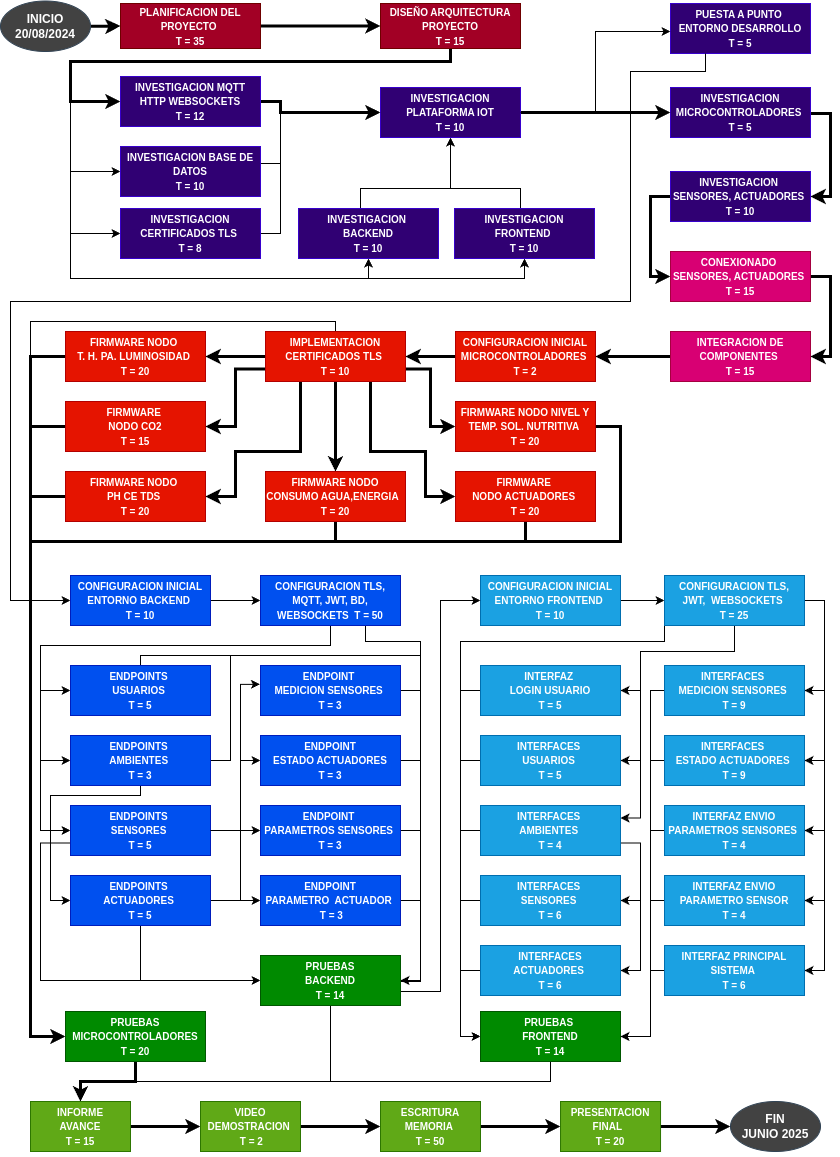
\includegraphics[width=.8\textwidth]{./Figuras/AoN.png}
\caption{Diagrama de \textit{Activity on Node}.}
\label{fig:AoN}
\end{figure}

Indicar claramente en qué unidades están expresados los tiempos.
De ser necesario indicar los caminos semi críticos y analizar sus tiempos mediante un cuadro.
Es recomendable usar colores y un cuadro indicativo describiendo qué representa cada color.

\end{consigna}

\section{11. Diagrama de Gantt}
\label{sec:gantt}

\begin{consigna}{red}
Existen muchos programas y recursos \textit{online} para hacer diagramas de Gantt, entre los cuales destacamos:

\begin{itemize}
\item Planner
\item GanttProject
\item Trello + \textit{plugins}. En el siguiente link hay un tutorial oficial: \\ \url{https://blog.trello.com/es/diagrama-de-gantt-de-un-proyecto}
\item Creately, herramienta online colaborativa. \\\url{https://creately.com/diagram/example/ieb3p3ml/LaTeX}
\item Se puede hacer en latex con el paquete \textit{pgfgantt}\\ \url{http://ctan.dcc.uchile.cl/graphics/pgf/contrib/pgfgantt/pgfgantt.pdf}
\end{itemize}

Pegar acá una captura de pantalla del diagrama de Gantt, cuidando que la letra sea suficientemente grande como para ser legible. 
Si el diagrama queda demasiado ancho, se puede pegar primero la ``tabla'' del Gantt y luego pegar la parte del diagrama de barras del diagrama de Gantt.

Configurar el software para que en la parte de la tabla muestre los códigos del EDT (WBS).\\
Configurar el software para que al lado de cada barra muestre el nombre de cada tarea.\\
Revisar que la fecha de finalización coincida con lo indicado en el Acta Constitutiva.

En la figura \ref{fig:gantt}, se muestra un ejemplo de diagrama de gantt realizado con el paquete de \textit{pgfgantt}. 
En la plantilla pueden ver el código que lo genera y usarlo de base para construir el propio.

Las fechas pueden ser calculadas utilizando alguna de las herramientas antes citadas. Sin embargo, el siguiente ejemplo
fue elaborado utilizando 
\href{https://docs.google.com/spreadsheets/d/1fBz8NhSpc4tkkhz3KjJCbh1nR_ltDkfEcZi4tZXduqs}{esta hoja de cálculo}.

Es importante destacar que el ancho del diagrama estará dado por la longitud del texto utilizado para las tareas 
(Ejemplo: tarea 1, tarea 2, etcétera) y el valor \textit{x unit}. Para mejorar la apariencia del diagrama, es necesario
ajustar este valor y, quizás, acortar los nombres de las tareas.

\begin{figure}[htpb]
  \begin{center}
    \begin{ganttchart}[
      time slot unit=day,
      time slot format=isodate,
      x unit=0.038cm,
      y unit title=0.7cm,
      y unit chart=0.6cm,
      milestone/.append style={xscale=4}
      ]{2021-03-05}{2021-12-16}
      \gantttitlecalendar*{2021-03-05}{2021-12-16}{year} \\
      \gantttitlecalendar*{2021-03-05}{2021-12-16}{month} \\
      \ganttgroup{Duración Total}{2021-03-05}{2021-12-16} \\
      %%%%%%%%%%%%%%%%%Organización
      \ganttgroup{Organización}{2021-03-05}{2021-04-16} \\
      \ganttbar{Planificación del proyecto}{2021-03-05}{2021-04-15} \\
      %%%%%%%%%%%%%%%%%Ejecución
      \ganttgroup{Ejecución}{2021-04-16}{2021-10-21} \\
      \ganttbar{Tarea 1}{2021-04-16}{2021-04-29} \\
      \ganttbar{Tarea 2}{2021-04-30}{2021-05-13} \\
      \ganttbar{Tarea 3}{2021-05-14}{2021-05-27} \\
      \ganttbar{Tarea 4}{2021-05-28}{2021-07-12} \\
      \ganttbar{Tarea 5}{2021-07-13}{2021-08-09} \\
      \ganttbar{Tarea 6}{2021-08-10}{2021-09-23} \\
      \ganttbar{Tarea 7}{2021-09-24}{2021-09-30} \\
      \ganttbar{Tarea 8}{2021-10-01}{2021-10-14} \\
      \ganttbar{Tarea 9}{2021-10-15}{2021-10-21} \\
      % %%%%%%%%%%%%%%%%%Finalización
      \ganttgroup{Finalización}{2021-10-22}{2021-12-16} \\
      \ganttbar{Memoria v1}{2021-10-22}{2021-11-04} \\
      \ganttbar{Memoria v2}{2021-11-05}{2021-11-18} \\
      \ganttbar{Memoria final}{2021-11-19}{2021-12-02} \\
      % La fecha del siguiente milestone es la fecha en que terminamos la memoria
      \ganttmilestone{Enviar memoria al director}{2021-12-02} \\
      \ganttbar{Elaborar la presentación}{2021-12-03}{2021-12-16} \\
      \ganttmilestone{Ensayo de la presentación}{2021-12-16} \\
      %%%%%%%%%%%%%%%%%%%%%%%%%%%%%%%%%%%%%%%%%%%%%%%%%%%%%%%%%%%%%%%
    \end{ganttchart}
  \end{center}
  \caption{Diagrama de gantt de ejemplo}
  \label{fig:gantt}
\end{figure}


\begin{landscape}
\begin{figure}[htpb]
\centering 
\includegraphics[height=.85\textheight]{./Figuras/Gantt-2.png}
\caption{Ejemplo de diagrama de Gantt (apaisado).} %Modificar este título acorde.
\label{fig:diagGantt}
\end{figure}

\end{landscape}

\end{consigna}


\section{12. Presupuesto detallado del proyecto}
\label{sec:presupuesto}

\begin{consigna}{red}
Si el proyecto es complejo entonces separarlo en partes:
\begin{itemize}
	\item Un total global, indicando el subtotal acumulado por cada una de las áreas.
	\item El desglose detallado del subtotal de cada una de las áreas.
\end{itemize}

IMPORTANTE: No olvidarse de considerar los COSTOS INDIRECTOS.

Incluir la aclaración de si se emplea como moneda el peso argentino (ARS) o si se usa moneda extranjera (USD, EUR, etc). Si es en moneda extranjera se debe indicar la tasa de conversión respecto a la moneda local en una fecha dada.

\end{consigna}

\begin{table}[htpb]
\centering
\begin{tabularx}{\linewidth}{@{}|X|c|r|r|@{}}
\hline
\rowcolor[HTML]{C0C0C0} 
\multicolumn{4}{|c|}{\cellcolor[HTML]{C0C0C0}COSTOS DIRECTOS} \\ \hline
\rowcolor[HTML]{C0C0C0} 
Descripción &
  \multicolumn{1}{c|}{\cellcolor[HTML]{C0C0C0}Cantidad} &
  \multicolumn{1}{c|}{\cellcolor[HTML]{C0C0C0}Valor unitario} &
  \multicolumn{1}{c|}{\cellcolor[HTML]{C0C0C0}Valor total} \\ \hline
 &
  \multicolumn{1}{c|}{} &
  \multicolumn{1}{c|}{} &
  \multicolumn{1}{c|}{} \\ \hline
 &
  \multicolumn{1}{c|}{} &
  \multicolumn{1}{c|}{} &
  \multicolumn{1}{c|}{} \\ \hline
\multicolumn{1}{|l|}{} &
   &
   &
   \\ \hline
\multicolumn{1}{|l|}{} &
   &
   &
   \\ \hline
\multicolumn{3}{|c|}{SUBTOTAL} &
  \multicolumn{1}{c|}{} \\ \hline
\rowcolor[HTML]{C0C0C0} 
\multicolumn{4}{|c|}{\cellcolor[HTML]{C0C0C0}COSTOS INDIRECTOS} \\ \hline
\rowcolor[HTML]{C0C0C0} 
Descripción &
  \multicolumn{1}{c|}{\cellcolor[HTML]{C0C0C0}Cantidad} &
  \multicolumn{1}{c|}{\cellcolor[HTML]{C0C0C0}Valor unitario} &
  \multicolumn{1}{c|}{\cellcolor[HTML]{C0C0C0}Valor total} \\ \hline
\multicolumn{1}{|l|}{} &
   &
   &
   \\ \hline
\multicolumn{1}{|l|}{} &
   &
   &
   \\ \hline
\multicolumn{1}{|l|}{} &
   &
   &
   \\ \hline
\multicolumn{3}{|c|}{SUBTOTAL} &
  \multicolumn{1}{c|}{} \\ \hline
\rowcolor[HTML]{C0C0C0}
\multicolumn{3}{|c|}{TOTAL} &
   \\ \hline
\end{tabularx}%
\end{table}


\section{13. Gestión de riesgos}
\label{sec:riesgos}

\begin{consigna}{red}
a) Identificación de los riesgos (al menos cinco) y estimación de sus consecuencias:
 
Riesgo 1: detallar el riesgo (riesgo es algo que si ocurre altera los planes previstos de forma negativa)
\begin{itemize}
	\item Severidad (S): mientras más severo, más alto es el número (usar números del 1 al 10).\\
	Justificar el motivo por el cual se asigna determinado número de severidad (S).
	\item Probabilidad de ocurrencia (O): mientras más probable, más alto es el número (usar del 1 al 10).\\
	Justificar el motivo por el cual se asigna determinado número de (O). 
\end{itemize}   

Riesgo 2:
\begin{itemize}
	\item Severidad (S): X.\\
	Justificación...
	\item Ocurrencia (O): Y.\\
	Justificación...
\end{itemize}

Riesgo 3:
\begin{itemize}
	\item Severidad (S):  X.\\
	Justificación...
	\item Ocurrencia (O): Y.\\
	Justificación...
\end{itemize}


b) Tabla de gestión de riesgos:      (El RPN se calcula como RPN=SxO)

\begin{table}[htpb]
\centering
\begin{tabularx}{\linewidth}{@{}|X|c|c|c|c|c|c|@{}}
\hline
\rowcolor[HTML]{C0C0C0} 
Riesgo & S & O & RPN & S* & O* & RPN* \\ \hline
       &   &   &     &    &    &      \\ \hline
       &   &   &     &    &    &      \\ \hline
       &   &   &     &    &    &      \\ \hline
       &   &   &     &    &    &      \\ \hline
       &   &   &     &    &    &      \\ \hline
\end{tabularx}%
\end{table}

Criterio adoptado: 

Se tomarán medidas de mitigación en los riesgos cuyos números de RPN sean mayores a...

Nota: los valores marcados con (*) en la tabla corresponden luego de haber aplicado la mitigación.

c) Plan de mitigación de los riesgos que originalmente excedían el RPN máximo establecido:
 
Riesgo 1: plan de mitigación (si por el RPN fuera necesario elaborar un plan de mitigación).
  Nueva asignación de S y O, con su respectiva justificación:
  \begin{itemize}
	\item Severidad (S*): mientras más severo, más alto es el número (usar números del 1 al 10).
          Justificar el motivo por el cual se asigna determinado número de severidad (S).
	\item Probabilidad de ocurrencia (O*): mientras más probable, más alto es el número (usar del 1 al 10).
          Justificar el motivo por el cual se asigna determinado número de (O).
	\end{itemize}

Riesgo 2: plan de mitigación (si por el RPN fuera necesario elaborar un plan de mitigación).
 
Riesgo 3: plan de mitigación (si por el RPN fuera necesario elaborar un plan de mitigación).

\end{consigna}


\section{14. Gestión de la calidad}
\label{sec:calidad}

\begin{consigna}{red}
Elija al menos diez requerimientos que a su criterio sean los más importantes/críticos/que aportan más valor y para cada uno de ellos indique las acciones de verificación y validación que permitan asegurar su cumplimiento.

\begin{itemize} 
\item Req \#1: copiar acá el requerimiento con su correspondiente número.

\begin{itemize}
	\item Verificación para confirmar si se cumplió con lo requerido antes de mostrar el sistema al cliente. Detallar.
	\item Validación con el cliente para confirmar que está de acuerdo en que se cumplió con lo requerido. Detallar. 
\end{itemize}

\end{itemize}

Tener en cuenta que en este contexto se pueden mencionar simulaciones, cálculos, revisión de hojas de datos, consulta con expertos, mediciones, etc.  

Las acciones de verificación suelen considerar al entregable como ``caja blanca'', es decir se conoce en profundidad su funcionamiento interno.  

En cambio, las acciones de validación suelen considerar al entregable como ``caja negra'', es decir, que no se conocen los detalles de su funcionamiento interno.

\end{consigna}

\section{15. Procesos de cierre}    
\label{sec:cierre}

\begin{consigna}{red}
Establecer las pautas de trabajo para realizar una reunión final de evaluación del proyecto, tal que contemple las siguientes actividades:

\begin{itemize}
	\item Pautas de trabajo que se seguirán para analizar si se respetó el Plan de Proyecto original:\\
	 - Indicar quién se ocupará de hacer esto y cuál será el procedimiento a aplicar. 
	\item Identificación de las técnicas y procedimientos útiles e inútiles que se emplearon, los problemas que surgieron y cómo se solucionaron:\\
	 - Indicar quién se ocupará de hacer esto y cuál será el procedimiento para dejar registro.
	\item Indicar quién organizará el acto de agradecimiento a todos los interesados, y en especial al equipo de trabajo y colaboradores:\\
	  - Indicar esto y quién financiará los gastos correspondientes.
\end{itemize}

\end{consigna}

\end{document}